% !TEX root = ../AiiDA_tutorial.tex
%%%%%%%%%%%%%%%%This slot is devoted to workflows, although the material inherited from the old tutorial does not use them.
% Nevertheless, it has been suggested to use workflows for calculating equation of state, so all this stuff can be inspirational 
%%%%%%%%%%%%%%%%%%%%%%

\section{AiiDA Workflows: workfunctions, workchains}

The aim of the last part of this tutorial is to introduce the concept of workflows in AiiDA. 

In this section, we will ask you to:
\begin{enumerate}
\item Understand how to keep the provenance when running small python scripts to convert one data object into another (postprocessing, preparation of inputs, \ldots)
\item Understand how to represent simple python functions in the AiiDA database
\item Learn how to write a simple workflow in AiiDA (without and with remote calculation submission)
\item Learn how to write a workflow with checkpoints: this means that, even if your
workflows requires external calculations to start, them and their dependences are managed through the daemon. While you are waiting for the calculations to complete, you can stop and even shutdown the computer in which AiiDA is running. When you restart, the workflow will
continue from where it was.
\item (optional) Go a bit deeper in the syntax of workflows with checkpoints (WorkChain), e.g. implementing a convergence workflow using \texttt{while} loops.
\end{enumerate}

A note: this is probably the most ``complex'' part of the tutorial.
We suggest that you try to understand the underlying logic behind the scripts,
without focusing too much on the details of the workflows implementation or the syntax.
If you want, you can then focus more on the technicalities in a second reading.

\subsection[Workfunctions]{Introduction}
The ultimate aim of this section is to create a workflow to calculate the equation of state of silicon. This is a very common task for an \textit{ab initio} researcher. An equation of state consists in calculating the total energy $E$ as a function of the unit cell volume $V$. The minimal energy is reached at the equilibrium volume $V^{\star}$. Equivalently, the equilibrium is defined by a vanishing pressure $p=-dE/dV$. In the vicinity of the minimum, the functional form of the equation of state can be approximated by a parabola. Such an approximation greatly simplifies the calculation of the bulk modulus, that is proportional to the second derivative of the energy $d^2E/dV^2$ (a more advanced treatment requires fitting the curve with, e.g., the Birch--Murnaghan expression).

The process of calculating an equation of state puts together several operations. 
First, we need to define and store in the AiiDA database the basic structure of, e.g., bulk Si.
Next, one has to define several structures with different lattice parameters. Those structures must be connected between them in the database, in order to ensure that their provenance is recorded. In other words, we want to be sure that in the future we will know that if we find a bunch of rescaled structures in the database, they all descend from the same one. How to link two nodes in the database in a easy way is the subject of Sec.~\ref{sec:provenancewf}.

In the following sections, the newly created structures will then serve as an input for total energy calculations performed, in this tutorial, with Quantum ESPRESSO. This task is very similar to what you have done in the previous part of the tutorial. Finally, you will fit the resulting energies as a function of volume to get the bulk modulus.
As the EOS task is very common, we will show how to automate its computation with workflows, and how to deal with both serial and parallel (i.e., independent) execution of multiple tasks. Finally, we will show how to introduce more complex logic in your workflows such as loops and conditional statements (Sec.~\ref{sec:convpressure}), with an example on a convergence loop to find iteratively the minimum of an EOS.


\subsection[Workfunctions]{\label{sec:provenancewf}Workfunctions: a way to generalize provenance in AiiDA}


%Figure with workfunction graph
\begin{figure}[!th]
\centering
 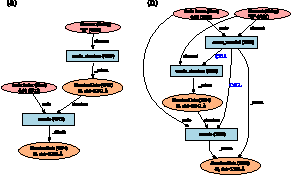
\includegraphics[width=\linewidth]{img/workfunctions}
 \caption{ \label{Fig:workfunctions}Typical graphs created by using a workfunction. (a) The workfunction ``create\_structure'' takes a \texttt{Str} object as input and returns a single \texttt{StructureData} object which is used as input for the workfunction ``rescale'' together with a \texttt{Float} object. This latter workfunction returns another \texttt{StructureData} object, defining a crystal having the rescaled lattice constant. (b) Graph generated by nesting workfunctions. A wrapper workfunction ``create\_rescaled" calls serially ``create\_structure'' and ``rescale". This relationship is stored via ``CALL'' links.}
\end{figure}


Imagine to have a function that takes as input a string of the name of a chemical element and generates the corresponding bulk structure as a \texttt{StructureData} object. The function might look like this (you will find this function in the folder \texttt{/home/aiida/tutorial\_scripts/create\_rescale.py} on your virtual machine):

\begin{pythoncommand}
def create_diamond_fcc(element):
    """
    Workfunction to create the crystal structure of a given element.
    For simplicity, only Si and Ge are valid elements.
    :param element: The element to create the structure with.
    :return: The structure.
    """
    import numpy as np
    elem_alat= {
                "Si": 5.431, # Angstrom
                "Ge": 5.658,
               }

    # Validate input element
    symbol = str(element)
    if symbol not in elem_alat.keys():
       raise ValueError("Valid elements are only Si and Ge")

    # Create cel starting having lattice parameter alat corresponding to the element
    alat = elem_alat[symbol]
    the_cell = np.array([[0., 0.5, 0.5],
                         [0.5, 0., 0.5],
                         [0.5, 0.5, 0.]]) * alat

    # Create a structure data object
    StructureData = DataFactory("structure")
    structure = StructureData(cell=the_cell)
    structure.append_atom(position=(0., 0., 0.), symbols=str(element))
    structure.append_atom(position=(0.25*alat, 0.25*alat, 0.25*alat),
                          symbols=str(element))
    return structure
\end{pythoncommand}

For the equation of state you need another function that takes as input a \texttt{StructureData} object and a rescaling factor, and returns a \texttt{StructureData} object with the rescaled lattice parameter (you will find this function in the same file \texttt{create\_rescale.py} on your virtual machine):

\begin{pythoncommand}
def rescale(structure, scale):
    """
    Workfunction to rescale a structure

    :param structure: An AiiDA structure to rescale
    :param scale: The scale factor (for the lattice constant)
    :return: The rescaled structure
    """
    the_ase = structure.get_ase()
    new_ase = the_ase.copy()
    new_ase.set_cell(the_ase.get_cell() * float(scale), scale_atoms=True)
    new_structure = DataFactory('structure')(ase=new_ase)
    return new_structure
\end{pythoncommand}

In order to generate the rescaled starting structures, say for five different lattice parameters you would combine the two functions. Enter the following commands in the \texttt{verdi shell} from the \texttt{tutorial\_scripts} folder.  

\begin{pythoncommand}
from create_rescale import create_diamond_fcc, rescale

s0 = create_diamond_fcc("Si")
rescaled_structures = [rescale(s0, factor) for factor 
                      in (0.98, 0.99, 1.0, 1.1, 1.2)]
\end{pythoncommand}

and store them in the database:

\begin{pythoncommand}
s0.store()
for struct in rescaled_structures:
   struct.store()
\end{pythoncommand}

\begin{tcolorbox}
Run the commands above to store all the structures.
\end{tcolorbox}

As expected, all the structures that you have created are not linked in any manner as you can verify via the \cmd{get\_inputs()/get\_outputs()} methods of the StuctureData class.
Instead, you would like these objects to be connected as sketched in Fig.~\ref{Fig:workfunctions}a. Now that you are familiar with AiiDA, you know that the way to connect two data nodes is through a calculation.
%However, you do not want to run such simple python functions on a cluster! Rather, you would like to simply run  them as simple python functions, but keep at the same time the provenance.
In order to ``wrap'' python functions and automate the generation of the
needed links, in AiiDA we provide you with what we call ``workfunctions''. A normal function can be converted to a workfunction by using the \texttt{@workfunction} decorator\footnote{In simple (or even simplified) words, a decorator is a function that modifies the behavior of another function. In python, a function can be decorated by adding a line of the form \texttt{@decorating\_function\_name} on the line just before the \texttt{def} line of the decorated function. If you want to know more, there are many online resources explaining python decorators.} that takes care of storing the execution as a calculation and adding the links between the input and output data nodes.

\begin{tcolorbox}
In our case, what you need to do is to modify the two functions as follows (note that we import \texttt{workfunction} as \texttt{wf} to be shorter, but this is not required). You can do it in the file \texttt{create\_rescale.py}:
\end{tcolorbox}

\begin{pythoncommand}
# Add this import
from aiida.work import workfunction as wf
 
# Add decorators
@wf
def create_diamond_fcc(element):
    ...
    ...
 
@wf
def rescale(structure, scale):
    ...
    ...
\end{pythoncommand}

\emph{Important}: when you use workfunctions, you have to make sure that their input and output are actually Data nodes, so that they can be stored in the database. AiiDA objects such as \texttt{StructureData}, ParameterData, etc.\@ carry around information about their provenance as stored in the database. This is why we must use the special database-storable types Float, Str, etc.\@ as shown in the snippet below.

\begin{tcolorbox}
Try now to run the following script:
\end{tcolorbox}
\begin{pythoncommand}
from aiida.orm.data.base import Float, Str
from create_rescale import create_diamond_fcc, rescale

s0 = create_diamond_fcc(Str("Si"))
rescaled_structures = [rescale(s0,Float(factor)) for factor in (0.98, 0.99, 1.0, 1.1, 1.2)]
\end{pythoncommand}
and check now that the output of \texttt{s0} as well as the input of the rescaled structures point to an intermediate ProcessCalculation node, representing the execution of the
workfunction, see Fig.~\ref{Fig:workfunctions}. 
\begin{tcolorbox}
For instance, you can check that the output links of \texttt{s0} are the five \texttt{rescale} calculations:
\end{tcolorbox}
\begin{pythoncommand}
s0.get_outputs()
\end{pythoncommand}
which outputs
\begin{pythoncommand}
[<FunctionCalculation: uuid: 01b0b137-974c-4d80-974f-ea4978b12019 (pk: 4970)>,
 <FunctionCalculation: uuid: 1af5ead6-0ae0-42a7-969c-1f0e88300f4a (pk: 4973)>,
 <FunctionCalculation: uuid: 22dee9d5-0382-48a3-9319-e800506946f1 (pk: 4976)>,
 <FunctionCalculation: uuid: dc4c93b7-3e7a-4f51-8d44-cf15c5707ddb (pk: 4979)>,
 <FunctionCalculation: uuid: f5b4e9f2-0d50-4b3d-a76b-7a12d232ea54 (pk: 4982)>]
\end{pythoncommand}
\begin{tcolorbox}
and the inputs of each ProcessCalculation (``rescale'') are obtained with:
\end{tcolorbox}
\begin{pythoncommand}
for s in s0.get_outputs():
     print s.get_inputs()
\end{pythoncommand}
that will return
\begin{pythoncommand}    
[0.98, <StructureData: uuid: 9b76b5fa-2908-4f88-a4fb-7a9aa343a1f3 (pk: 4968)>]
[0.99, <StructureData: uuid: 9b76b5fa-2908-4f88-a4fb-7a9aa343a1f3 (pk: 4968)>]
[1.0, <StructureData: uuid: 9b76b5fa-2908-4f88-a4fb-7a9aa343a1f3 (pk: 4968)>]
[1.1, <StructureData: uuid: 9b76b5fa-2908-4f88-a4fb-7a9aa343a1f3 (pk: 4968)>]
[1.2, <StructureData: uuid: 9b76b5fa-2908-4f88-a4fb-7a9aa343a1f3 (pk: 4968)>]
\end{pythoncommand}

\subsubsection{Workfunction nesting}
One key advantage of workfunctions is that they can be nested, namely, a workfunction can invoke workfunctions inside its definition, and this ``call'' relationship will also be automatically recorded in the database. 
As an example, let us combine the two previously defined workfunctions by means of a wrapper workfunction called ``create\_rescaled'' that takes as input the element and the rescale factor.
\begin{tcolorbox}
Type in your shell (or modify the functions defined in \texttt{create\_rescale.py} and then run):
\end{tcolorbox}
%%%%%%%%%%Call link
\begin{pythoncommand}
@wf
def create_rescaled(element, scale):
    """
    Workfunction to create and immediately rescale
    a crystal structure of a given element.
    """
    s0 = create_diamond_fcc(element)
    return rescale(s0,scale)
\end{pythoncommand}
and create an already rescaled structure by typing 
\begin{pythoncommand}
s1 = create_rescaled(element=Str("Si"), scale=Float(0.98))
\end{pythoncommand}
\begin{tcolorbox}
Now inspect the input links of \texttt{s1}:
\end{tcolorbox}
\begin{pythoncommand}
In [6]: s1.get_inputs()
Out[6]: 
[<FunctionCalculation: uuid: a672317b-3091-4135-9d84-12c2fff34bfe (pk: 5005)>,
 <FunctionCalculation: uuid: a672317b-3091-4135-9d84-12c2fff34bfe (pk: 5005)>,
 <FunctionCalculation: uuid: f64f4a70-70ff-4551-ba4d-c186328d8bd6 (pk: 5002)>]
\end{pythoncommand}

The object \texttt{s1} has three incoming links, corresponding to \emph{two} different calculations as input (in this case, pks 5002 and 5005). These correspond to the calculations ``create\_rescaled'' and ``rescale'' as shown in Fig.~\ref{Fig:workfunctions}b.
It is normal that calculation 5005 has two links, don't worry about that\footnote{If you are curious: the two links have the same label, but are of different \emph{link\_type}: one is a \textbf{create} link, that keeps track of the calculation that actually generated the node. Instead the other one is of type \textbf{return}, stating that the workfunction, beside creating that node, also returned it as an output. Calculation 5002 instead only returned the node but it did not generate it, therefore there is only one link between it and the final \texttt{StructureData}.}.
To see the ``call'' link, inspect now the outputs of the calculation appearing only once in the list. Write down its \texttt{<pk>} (in general, it will be different from 5002), then in the shell load the corresponding node and inspect the outputs:
\begin{pythoncommand}
In [12]: p1 = load_node(<pk>)
In [13]: p1.get_outputs_dict()
\end{pythoncommand}
\begin{tcolorbox}
You should be able to identify the two ``children" calculations as well as the final structure (you will see the calculations linked via CALL links: these are calculation-to-calculation links representing the fact that \texttt{create\_rescaled} called two sub-workfunctions). The graphical representation of what you have in the database should match Fig.~\ref{Fig:workfunctions}b.  
\end{tcolorbox}

\subsection{\label{sec:sync} Run a simple workflow}

Let us now use the workfunctions that we have just created to build a simple workflow to calculate the equation of state of silicon. We will consider five different values of the lattice parameter obtained rescaling the experimental minimum, $a=5.431~\text{\AA}$, by a factor in $[0.96, 0.98, 1.0, 1.02, 1.04]$. We will write a simple script that runs a series of five calculations and at the end returns the volume and the total energy corresponding to each value of the lattice parameter. For your convenience, besides the functions that you have written so far in the file \texttt{create\_rescale.py}, we provide you with some other utilities to get the correct pseudopotential and to generate a pw input file, in the module \texttt{common\_wf.py} which has been put in the \texttt{tutorial\_scripts} folder.

\begin{tcolorbox}
We have already created the following script named \texttt{simple\_sync\_workflow.py}, which you are free to look at but please go through the lines carefully and make sure you understand them.
If you decide to create your own new script, make sure to also place it in the folder \texttt{tutorial\_scripts}, otherwise the imports won't work.
\end{tcolorbox}
Besides the functions in the local folder
\begin{pythoncommand}
from create_rescale import create_diamond_fcc, rescale
from common_wf import generate_scf_input_params
\end{pythoncommand}
you need to import few further AiiDA classes and functions:
\begin{pythoncommand}
from aiida.work import run, Process
from aiida.work import workfunction as wf
from aiida.orm.data.base import Str, Float
from aiida.orm import CalculationFactory, DataFactory
\end{pythoncommand}

The only imported function that deserves an explanation is \texttt{run}.
For the time being, you just need to know that it is a function that needs to be used to execute a new workflow.
The actual body of the script is the following.
We suggest that you first have a careful look at it before running it.

\begin{pythoncommand}
# Load the calculation class 'PwCalculation' using its entry point 'quantumespresso.pw'
PwCalculation = CalculationFactory('quantumespresso.pw')

scale_facs = (0.96, 0.98, 1.0, 1.02, 1.04)
labels = ["c1", "c2", "c3", "c4", "c5"]

@wf
def run_eos_wf(codename, pseudo_family, element):
    print "Workfunction node identifiers: {}".format(Process.current().calc)
    s0 = create_diamond_fcc(Str(element))

    calcs = {}
    for label, factor in zip(labels, scale_facs):
        s = rescale(s0, Float(factor))
        inputs = generate_scf_input_params(s, str(codename), Str(pseudo_family))
        print "Running a scf for {} with scale factor {}".format(element, factor)
        result = run(PwCalculation, **inputs)
        print "RESULT: {}".format(result)
        calcs[label] = get_info(result)

    eos = []
    for label in labels:
        eos.append(calcs[label])

    # Return information to plot the EOS
    ParameterData = DataFactory("parameter")
    retdict = {
            'initial_structure': s0,
            'result': ParameterData(dict={'eos_data': eos})
        }

    return retdict
\end{pythoncommand}

If you look into the previous snippets of code, you will notice that the way we submit a QE calculation is slightly different from what you have seen in the first part of the tutorial.  The following:
\begin{pythoncommand}
result = run(PwCalculation, **inputs)
\end{pythoncommand}
runs in the current python session (without the daemon), waits for its completion and returns the output in the user-defined variable \texttt{result}.
The latter is a dictionary whose values are the output nodes generated by the calculation, with the link labels as keys.
For example, once the calculation is finished, in order to access the total energy, we need to access the ParameterData node which is linked via the ``output\_parameters'' link (see again Fig.~1 of Day 1 Tutorial, to see inputs and outputs of a Quantum ESPRESSO calculation).
Once the right node is retrieved as \cmd{result[`output\_parameters']}, we need to get the \texttt{energy} attribute. The global operation is achieved by the command
\begin{pythoncommand}
result['output_parameters'].dict.energy
\end{pythoncommand}
As you see, the function \texttt{run\_eos\_wf} has been decorated as a workfunction to keep track of the provenance.
Finally, in order to get the \texttt{<pk>} associated to the workfunction (and print on the screen for our later reference), we have used the following command to get the node corresponding to the ProcessCalculation:
\begin{pythoncommand}
from aiida.work import Process
print Process.current().calc
\end{pythoncommand}

To run the workflow it suffices to call the function \texttt{run\_eos\_wf} in a python script providing the required input parameters. For simplicity, we have included few lines at the end of the script that invoke the function with a static choice of parameters: 

\begin{pythoncommand}
def run_eos(codename='pw-5.1@localhost', pseudo_family='GBRV_lda', element="Si"):
    return run_eos_wf(Str(codename), Str(pseudo_family), Str(element))

if __name__ == '__main__':
    run_eos() 
\end{pythoncommand}

\begin{tcolorbox}
Run the workflow by running the following command from the \texttt{tutorial\_scripts} directory:
\begin{bashcommand}
verdi run simple_sync_workflow.py
\end{bashcommand}
and write down the \texttt{<pk>} of the ProcessCalculation printed on screen at execution.
\end{tcolorbox}

The command above locks the shell until the full workflow has completed (we will see in a moment how to avoid this).
While the calculation is running, you can use (in a different shell) the command \cmd{verdi work list} to show ongoing and finished workfunctions. You can ``grep'' for the \texttt{<pk>} you are interested in. Additionally, you can use the command \cmd{verdi work status <pk>}  to show the tree of the sub-workfunctions called by the root workfunction with a given \texttt{<pk>}.

\begin{tcolorbox}
Wait for the calculation to finish, then call the function \cmd{plot\_eos(<pk>)} that we provided in the file \texttt{common\_wf.py} to plot the equation of state and fit it with a Birch--Murnaghan equation.
\end{tcolorbox}

\subsection{\label{sec:wf-multiple-calcs}Run multiple calculations}

You should have noticed that the calculations for different lattice parameters are executed serially, although they might perfectly be executed in parallel because their inputs and outputs are not connected in any way.
In the language of workflows, these calculations are executed in a synchronous (or blocking) way, whereas we would like to have them running \emph{asynchronously} (i.e., in a non-blocking way, to run them in parallel). 
One way to achieve this to submit the calculation to the daemon using the \cmd{submit} function.
Make a copy of the script \texttt{simple\_sync\_workflow.py} that we worked on in the previous section and name it \texttt{simple\_submit\_workflow.py}.
To make the new script work asynchronously, simply change the following subset of lines:
\begin{pythoncommand}
from aiida.work import run
[...]
for label, factor in zip(labels, scale_facs):
    [...]
    result = run(PwCalculation, **inputs)
    calcs[label] = get_info(result)
[...]
eos = []
for label in labels:
    eos.append(calcs[label])
\end{pythoncommand}
replacing them with
\begin{pythoncommand}
from aiida.work import submit
from time import sleep
[...]
for label, factor in zip(labels, scale_facs):
    [...]
    calcs[label] = submit(PwCalculation, **inputs)
[...]
# Wait for the calculations to finish
for calc in calcs.values():
    while not calc.is_finished:
        sleep(1)

eos = []
for label in labels:
    eos.append(get_info(calcs[label].get_outputs_dict()))
\end{pythoncommand}

The main differences are:
\begin{itemize}
 \item \cmd{run} is replaced by \cmd{submit}
 \item The return value of \texttt{submit} is not a dictionary describing the outputs of the calculation, but it is the calculation node for that submission.
 \item Each calculation starts in the background and calculation nodes are added to the \texttt{calc} dictionary.
 \item At the end of the loop, when all calculations have been launched with \cmd{submit}, another loop is used to wait for all calculations to finish before gathering the results as the final step.
 
\end{itemize}
In the next section we will show you another way to achieve this, which has the added bonus that it introduces checkpoints in the workfunction, from which the calculation can be resumed should it be interrupted.

\begin{tcolorbox}
After applying the modifications, run the script. You will see that all calculations start at the same time, without waiting for the previous ones to finish.
\end{tcolorbox}
If in the meantime you run \cmd{verdi work status <pk>}, all five calculations are already shown as output. Also, if you run \cmd{verdi calculation list}, you will see how the calculations are submitted to the scheduler.


\subsection{\label{sec:workchainsimple}Workchains, or how not to get lost if your computer shuts down or crashes}
The simple workflows that we have used so far have been launched by a python script that needs to be running for the whole time of the execution, namely the time in which the calculations are submitted, and the actual time needed by Quantum ESPRESSO to perform the calculation and the time taken to retrieve the results. 
If you had killed the main python process during this time, the workflow would not have terminated correctly.  Perhaps you have kill the calculation and you experienced the unpleasant consequences: intermediate calculation results are potentially lost and it is extremely difficult to restart a workflow from the exact place where it stopped.

In order to overcome this limitation, in AiiDA we have implemented a way to insert checkpoints, where the main code defining a workflow can be stopped (you can even shut down the machine on which AiiDA is running!). We call these workfunctions with checkpoints ``workchains'' because, as you will see, they basically amount to splitting a workfunction in a chain of steps. Each step is then ran by the daemon, in a way similar to the remote calculations.

The basic rules that allow you to convert your workfunction-based script to a workchain-based one are listed in Table~\ref{Tab:wf2frag}, which focus on the code used to perform the calculation of an equation of state. The modifications needed are put side-to-side to allow for a direct comparison. In the following, when referencing a specific part of the code we will refer to the line number appearing in Table~\ref{Tab:wf2frag}. 

\begin{sidewaystable}
\caption{\label{Tab:wf2frag}Side-to-side comparison of the EOS workflow using standard workfunctions (left panel) or ``workchains'' (right panel).}
\scriptsize
\begin{tabular}{|c|c|}
\hline
{Workfunctions}&
{Workchains}\\
\hline
{
\begin{lstlisting}[language=Python,numbers=left,moredelim={[is][\color{gray}]{??}{??}}]
from aiida.work import submit, Process
# ...













@wf
def run_eos_wf(codename, pseudo_family, element):
    # ...
    s0 = create_diamond_fcc(Str(element))
    
    
    calcs = {}
    for label, factor in zip(labels, scale_facs):
        s = rescale(s0,Float(factor))
        inputs = generate_scf_input_params(
            s, str(codename), pseudo_family)
        # ...
        calcs[label] = submit(PwCalculation, **inputs)

        
    # Wait for the calculations to finish
    for calc in calcs.values():
        while not calc.is_finished:
            sleep(1)

    eos = []
    for label in labels:
        eos.append(get_info(calcs[label].get_outputs_dict()))
    
    #Return information to plot the EOS
    ParameterData = DataFactory("parameter")
    retdict = {
            'initial_structure': s0,
            'result': ParameterData(dict={'eos_data': eos})
        }

    return retdict

\end{lstlisting}
} &
{
\begin{lstlisting}[language=Python,numbers=left,moredelim={[is][\color{gray}]{??}{??}}]
from aiida.work.workchain import WorkChain, ToContext
# ...

class EquationOfStates(WorkChain):
    @classmethod
    def define(cls, spec):
        super(EquationOfStates, cls).define(spec)
        spec.input('element', valid_type=Str)
        spec.input('code', valid_type=Str)
        spec.input('pseudo_family', valid_type=Str)
        spec.outline(
            cls.run_pw,
            cls.return_results,
        )


    def run_pw(self):
        # ...
        self.ctx.s0 = create_diamond_fcc(Str(self.inputs.element))


        calcs = {}
        for label, factor in zip(labels, scale_facs):
            s = rescale(self.ctx.s0,Float(factor))
            inputs = generate_scf_input_params(
                s, str(self.inputs.code), self.inputs.pseudo_family)
            # ...
            future = self.submit(PwCalculation, **inputs)
            calcs[label] = future
          
        # Ask the workflow to continue when the results are ready 
        # and store them in the context
        return ToContext(**calcs)

    def return_results(self):
        eos = []
        for label in labels:
            eos.append(get_info(self.ctx[label].get_outputs_dict()))

        # Return information to plot the EOS
        ParameterData = DataFactory('parameter')
        retdict = {
                'initial_structure': self.ctx.s0,
                'result': ParameterData(dict={'eos_data': eos})
           }
        for link_name, node in retdict.iteritems():
            self.out(link_name, node)

\end{lstlisting}
}
\\
\hline
\end{tabular}
\end{sidewaystable}


\begin{itemize}
 \item Instead of using decorated functions you need to define a class, inheriting from a prototype class called \cmd{WorkChain} that is provided by AiiDA (line 4)
 %
 \item Within your class you need to implement a \cmd{define} classmethod that always takes \texttt{cls} and \texttt{spec} as inputs. (lines 6--7). Here you specify the main information on the workchain, in particular:
 \begin{itemize}
 \item the \emph{inputs} that the workchain expects. This is obtained by means of the \text{spec.input()} method, which provides as the key feature the automatic validation of the input types via the \texttt{valid\_type} argument (lines 8--10). The same holds true for outputs, as you can use the \texttt{spec.output()} method to state what output types are expected to be returned by the workchain. Both \texttt{spec.input()} and \texttt{spec.output()} methods are optional, and if not specified, the workchain will accept any set of inputs and will not perform any check on the outputs, as long as the values are database storable AiiDA types.
 %
 \item the \cmd{outline} consisting in a list of ``steps'' that you want to run, put in the right sequence (lines 11--14). This is obtained by means of the method \cmd{spec.outline()} which takes as input the steps. \emph{Note}: in this example we just split the main execution in two sequential steps, that is, first \cmd{run\_pw} then \cmd{return\_results}. However, more complex logic is allowed, as will be explained in the Sec.~\ref{sec:convpressure}.
 \end{itemize}
 %
 \item You need to split your main code into methods, with the names you specified before into the outline (\cmd{run\_pw} and \cmd{return\_results} in this example, lines 17 and 35). Where exactly should you split the code? Well, the splitting points should be put where you would normally block the execution of the script for collecting results in a standard workfunction, namely whenever you call the method \cmd{.result()}. Each method should accept only one parameter, \texttt{self}, e.g. \cmd{def step\_name(self)}.
 %
 \item You will notice that the methods reference the attribute \cmd{ctx} through \cmd{self.ctx}, which is called the \emph{context} and is inherited from the base class \texttt{WorkChain}.
 A python function or workfunction normally just stores variables in the local scope of the function.
 For instance, in the example of the subsection~\ref{sec:sync}, you stored the \cmd{calc\_results} in the \cmd{eos} list, that was a local variable.
 In workchains, instead, to preserve variables between different steps, you need to store them in a special dictionary called \emph{context}.
 As explained above, the context variable \cmd{ctx} is inherited from the base class \texttt{WorkChain}, and at each step method you just need to update its content.
 AiiDA will take care of saving the context somewhere between workflow steps (on disk, in the database, \ldots{}, depending on how AiiDA was configured).
 For your convenience,  you can also access the value of a context variable as \cmd{self.ctx.varname} instead of \cmd{self.ctx['varname']} (see e.g. lines 19, 24, 38, 43).
 %
 \item Any submission within the workflow should not call the normal \cmd{run} or \cmd{submit} functions, but \cmd{self.submit} to which you have to pass the Process class, and a dictionary of inputs (line 28).
 %
 \item The submission in line 28, returns a future and not the actual calculation, because at that point in time we have only just launched the calculation to the daemon and it is not yet completed. Therefore it literally is a ``future'' result. Yet we still need to add these futures to the context, so that in the next step of the workchain, when the calculations are in fact completed, we can access them and continue the work. To do this, we can use the \texttt{ToContext} class. This class takes a dictionary, where the values are the futures and the keys will be the names under which the corresponding calculations will be made available in the context when they are done. See line 33 how the \texttt{ToContext} object is created and returned from the step.
 By doing this, the workchain will implicitly wait for the results of all the futures you have specified, and then call the next step \emph{only when all futures have completed}.
 %
 \item \emph{Return values}: While in a normal workfunction you attach output nodes to the \texttt{FunctionCalculation} by invoking the \textit{return} statement, in a workchain you need to call \cmd{self.out(link\_name, node)} for each node you want to return (line 46-47). Of course, if you have already prepared a dictionary of outputs, you can just use the following syntax:
\begin{pythoncommand}
self.out_many(retdict)  # Keys are link names, value the nodes
\end{pythoncommand}


The advantage of this different syntax is that you can start emitting output nodes already in the middle of the execution, and not necessarily at the very end as it happens for normal functions (\textit{return} is always the last instruction executed in a function). Also, note that once you have called \cmd{self.out(link\_name, node)} on a given \cmd{link\_name}, you can no longer call \cmd{self.out()} on the same \cmd{link\_name}: this will raise an exception.
\end{itemize}

Inspect the example in the table that compares the two versions of workfunctions to understand in detail the different syntaxes.

Finally, the workflow has to be run. For this you have to use the function \cmd{run} passing as arguments the \texttt{EquationOfStates} class and the inputs as key-value arguments. For example, you can execute

\begin{pythoncommand}
 run(EquationOfStates, element=Str('Si'), code=Str('qe-pw-6.2.1@localhost'),
     pseudo_family=Str('GBRV_lda'))
\end{pythoncommand}

While the workflow is running, you can check (in a different terminal) what is happening
to the calculations using \cmd{verdi calculation list}. You will see that after a few seconds the calculations are all submitted to the scheduler and can potentially run at the same time.

\begin{tcolorbox}
\textbf{Note:}
You will see warnings that say \texttt{`Exception trying to save checkpoint, this means you will not be able to restart in case of a crash until the next successful checkpoint'}, these are generated by the \texttt{PwCalculation} which is unable to save a checkpoint because it is not in a so called `importable path'.  Simply put this means that if AiiDA were to try and reload the class it wouldn't know which file to find it in.\\
To get around this you could simply put the workchain in a different file that is in the `PYTHONPATH' and then launch it by importing it in your launch file, this way AiiDA knows where to find it next time it loads the checkpoint.
\end{tcolorbox}

As an additional exercise (optional), instead of running the main workflow (\texttt{EquationOfStates}),
try to submit it. Note that the file where the WorkChain is defined will need to be globally importable (so the daemon knows how to load it) and you need to launch it (with \cmd{submit}) from a different python file. The easiest way to achieve this is typically to embed the workflow inside a python package.

\begin{tcolorbox}
\textbf{Note:} 
As good practice, you should try to keep the steps as short as possible in term of execution time. The reason is that the daemon can be stopped and restarted only between execution steps and not if a step is in the middle of a long execution.
\end{tcolorbox}

Finally, as an optional exercise if you have time, you can jump to the Appendix~\ref{sec:convpressure}, which shows how to introduce more complex logic into your WorkChains (if conditionals, while loops etc.). The exercise will show how to realize a convergence loop to obtain the minimum-volume structure in a EOS using the Newton's algorithm.
